% Obfuscation strategies: the three example strategies. Release rules from DESIGN_FACTS.md
% ("Release rules (T)"); response layouts from DESIGN_FACTS.md ("Response-size normalization").
\section{Obfuscation Strategies}
\label{sec:strategies}

NOMAD applies a strategy per type of operation rather than per packet. In this section, we present three example strategies, which together cover the timing and size features of the two transactions in Fig.~\ref{fig:ladder}: a timing replacement for READ and SELECT, a hold for OPERATE, and a response layout that splits control units. Each strategy is a policy installed by the control plane on the infrastructure of Section~\ref{sec:infrastructure}.

\subsection{Strategy 1: Replacing the Read-Lane Timing}

\textbf{Timing model.} In Fig.~\ref{fig:timeline}(a), we show the timing of a READ transaction. We denote the arrival time of the request at the switch by $t_0$, the arrival times of the acknowledgment and the response by $t_A$ and $t_R$, and the times they depart toward the master by $e_A$ and $e_R$. Without NOMAD, the master measures
\begin{equation}
\label{eq:clrt-original}
\mathrm{CLRT}_{\mathrm{original}} = t_R - t_A ,
\end{equation}
which follows how long the outstation takes to answer.

\textbf{Replacing the interval.} A constant hold on each packet would only shift $\mathrm{CLRT}_{\mathrm{original}}$, and the variation that a timing classifier uses would survive the shift. To remove that variation, we anchor both departures to the request and to the acknowledgment's own release: the switch releases the acknowledgment once a deadline $d_a$ after the request has passed and the response of the same transaction has arrived, and it releases the response a configured interval $D$ after the acknowledgment:
\begin{equation}
\label{eq:release}
e_A = \max(t_0 + d_a,\; t_R), \qquad e_R = e_A + D .
\end{equation}
Consequently, the interval the master measures becomes
\begin{equation}
\label{eq:clrt-new}
e_R - e_A = D ,
\end{equation}
independent of the values of $t_A$ and $t_R$, as long as the response arrives before the acknowledgment's deadline. A response that arrives early waits longer, and one that arrives close to the deadline waits less. The two holds, $e_A - t_A$ and $e_R - t_R$, are not configured; the schedule determines them. SELECT, the first half of a select-before-operate control, follows the same rule.

\begin{figure}[t]
\centering
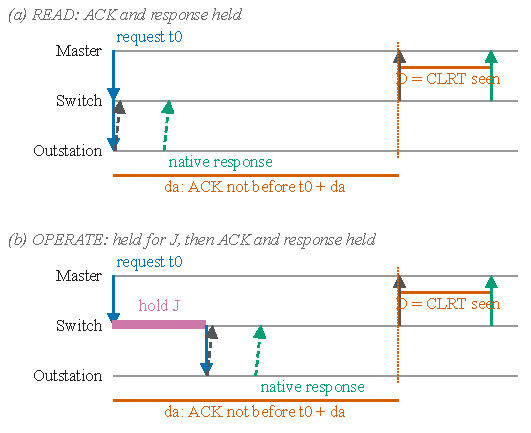
\includegraphics[width=\columnwidth]{figures/nomad/fig_nomad_timeline}
\caption{Release timeline at $D$ = 10~ms and $J$ = 10~ms, placed at campaign medians. (a) READ: the switch holds the acknowledgment until $d_a$ after the request and releases the response $D$ after it. (b) OPERATE: the switch first holds the command for $J$, then holds the acknowledgment and the response exactly as in (a).}
\label{fig:timeline}
\end{figure}

\textbf{Release in practice.} The actual release adds the time for the blocker tokens of the held packet to drain and for the scheduler to serve it, which is at most one recirculation pass after the deadline. If the response has not arrived by a later fallback deadline (Section~\ref{sec:objectives}), the switch releases what it holds rather than waiting indefinitely.

\subsection{Strategy 2: Holding Control Operations}

The OPERATE half of a select-before-operate control carries the physical execution of a command, which Formby et al.\ use as a second fingerprint~\cite{formby2016}. To separate the timing of the operation from its arrival, we hold each OPERATE command at the switch for a configured interval $J$ before it delivers the command to the outstation. The acknowledgment and the response of OPERATE then follow Strategy~1 with the same anchor $t_0$, the OPERATE's arrival at the switch, as shown in Fig.~\ref{fig:timeline}(b). Because the outstation sees the command only after $J$, its response arrives near $t_0 + J + L$, where $L$ is the time the outstation takes to respond. As long as $d_a \geq J + L$, the acknowledgment still leaves at $t_0 + d_a$ and the response at $e_A + D$, and the master-facing link reveals neither the hold nor the device's execution time. This condition is one of the constraints of Section~\ref{sec:objectives}.

\subsection{Strategy 3: Splitting Control Units}

Responses of different operations differ in size, and the size alone can reveal the operation. In our testbed, a READ response carries 49~bytes of TCP payload and a SELECT or OPERATE response carries 37~bytes. Padding such a response with filler would either break the DNP3 syntax or expose the filler to an observer who parses the plain text. We, on the other hand, change the layout of the control units the response already carries, using the index syntax of Section~\ref{sec:background}.

\textbf{READ responses.} In our testbed, the native READ response returns 23 binary output status points (object group 10, variation 2), indices 0 to 22, in one object header. We re-encode the same points as three consecutive index ranges, 0--5 and 6--9 with one-byte start and stop indices and 10--22 with two-byte indices. Every value appears once, in the same order, and the response grows to 61~bytes.

\textbf{SELECT and OPERATE responses.} The 22 application bytes of the native response are split as 15, 6 and 1 bytes across three DNP3 transport frames of 28, 19 and 14~bytes, which travel in one TCP segment of 61~bytes. The master's DNP3 stack reassembles the three frames into the original application fragment.

In both cases, a normalized response carries 61~bytes, the master receives the same control units in the same order, and every frame keeps valid CRCs and transport sequence numbers. Requests stay as the master sent them; NOMAD normalizes the responses only.
